\section*{Format danych PGN}
Fromat PGN jest powszechnie stosowanym sposobem pechowywania partii szachowych. W danym pliku może znajdować się dowolna ilość gier. Każda z nich ma między innymi nazwy graczy, wynik oraz stos ruchów. Taki sposób zapisu jest bardzo efektywny pamięciowo, gdyż nie zapisuje on pozycji na planszy w każdej turze, a jedynie wykonywane ruchy. Dodatkowym atutem jest gotowa biblioteka python-chess\footnote{https://python-chess.readthedocs.io/} do dekodowania pliku oraz rozgrywania partii.

\vspace{0.5cm}

\begin{lstlisting}[
    language=Python, 
    caption=przykład pliku PGN,
    inputencoding=utf8,
    basicstyle=\ttfamily\footnotesize,
    xleftmargin=0.1cm,
    showspaces=false,
    showstringspaces=false,
    showtabs=false,
    keepspaces=true
]
[Event "F/S Return Match"] 
[Site "Belgrade, Serbia JUG"] 
[Date "1992.11.04"] 
[Round "29"] 
[White "Fischer, Robert J."]
[Black "Spassky, Boris V."] 
[Result "1/2-1/2"] 

1. e4 e5 2. Nf3 Nc6 3. Bb5 a6 4. Ba4 Nf6 5. O-O Be7 6. Re1 b5 7. Bb3 d6 ...
\end{lstlisting}
\section*{Przetwarzanie danych}
Dane użyte do wstępnego trenowania modelu zostały pobrane ze strony pgnmentor\footnote{https://www.pgnmentor.com/}. Przy ich pobieraniu brany był uwagę ranking graczy. Dane z zawodów nie były używane ze zwględu na różne niestandardowe układy figur na planszy, co wprowadzało błędy. Do przetworzenia danych została stworzona klasa PGNDataset. Jej zadaniem jest utworzenie plików o rozszerzeniu .rdg, które zawierają zserializowany obiekt krotki. Rozbicie danych gier na kilka plików zostało podyktowane ograniczeniami pamięci dynamicznej procesora oraz procesora graficznego. Każdy z nich zawiera z góry ustaloną ilość zakodowanych partii, dzięki czemu w prosty sposób można zarządzać wielkością pliku, a tym samym ilością zajętej pamięci graficznej, co ma bardzo duży wpływ na prędkość trenowania modelu. W przypadku za dużego pliku karta graficzna musi używać współdzielonej pamięci, co znacznie spowalnia proces trenowania ze względu na konieczność przesyłania danych pomiędzy pamięcią ram, a vram. W przypadku zbyt małych plików, podczas procesu trenowania trzeba często wczytywać dane z dysku do ramu \footnote{Systemy operacyjne są w stanie cache'ować często używane dane w pamięci dynamicznej. W dystrybucji Ubuntu można zauważyć w system monitorze pod nazwą "Cache"}, a następnie przesyłać je do karty, co również spowalnia cały proces.

\section*{Klasa PGNDataset}
Działanie klasy rozpoczyna się od metody \textit{encode directory}, która przyjmuje ścieżke do katalogu z plikami \textit{.pgn}. Następnie iteruje po wszystkich plikach. Dla każdej gry z pliku wywołuje metodę \textit{encode game}, której listing jest przedstawiony pod spodem. Enkoduje ona ruchy, plansze oraz wynik partii i zwraca je w postaci trzech tablic numpy. Po przetworzeniu odpowiedniej ilości gier, są one zapisywane do pliku \textit{.rdg} w postaci krotki. Dodatkowo ze względu na model, który uczy się jedynie ruchów dla białych figur, obracana jest plansza po przekątnej. Dzięki temu zmieniamy perspektywę gracza. Działa to identycznie tak jakbyśmy w rzeczywistości zamienili się miejscem z przeciwnikiem. W przypadku zmiany perspektywy planszy, również jest zmieniana perspektywa ruchu oraz odwracany jest wynik partii. 

\lstset{style=codeListingStyle}
\begin{lstlisting}[
    language=Python, 
    caption=Metoda encode game,
    inputencoding=utf8
]
def encode_game(self, game: chess.pgn.Game):
        board = BoardPlus()
        moves, boards, wins = [], [], []

        for move in game.mainline_moves():
            real_board.push(move)
            if board.changed_perspective:
                move = BoardPlus.change_move_perspective(move)

            moves.append(board.encode_move(move))
            boards.append(board.encode())
            wins.append(self.white_win(game) * (1 if not board.changed_perspective else -1))
            board.better_push(move)

            board.change_perspective()
        return np.array(moves), np.array(boards), np.array(wins)
\end{lstlisting}

\section*{Przechowywanie zakodowanych gier w pamięci programu}
Dane w postaci list zwracane przez metodę \textit{encode game} są dodawane do kolejnych trzech list \textit{games move}, \textit{games board} oraz \textit{games win}. Po przetworzeniu odpowiedniej ilości gier są one scalane za pomocą metody \textit{concatenate} i zapisywane do pliku. Taki nietypowy sposób przechowywania został zastosowany ze względów wydajnościowych. Przy użyciu jednowymiarowych list, po każdym wywołaniu metody \textit{enocde game}, trzeba by używać \textit{concatenate} do scalania danych, co jest bardzo nieefektywne. Wraz z wielkością list, czas wykonania rośnie znacząco co można zaobserwować na poniższym wykresie.

\lstset{style=codeListingStyle}
\begin{lstlisting}[
    language=Python, 
    caption=Fragment metody encode directory,
    inputencoding=utf8
]
game_moves, game_boards, game_wins = self.encode_game(game)

if len(game_moves) == 0 or len(game_boards) == 0 or len(game_wins) == 0:
    continue
games_move.append(game_moves)
games_board.append(game_boards)
games_win.append(game_wins)

PGNDataset.number_converted_games += 1
if PGNDataset.number_converted_games % max_games_in_file == 0:
    moves, boards, wins = np.concatenate(games_move), np.concatenate(games_board), np.concatenate(games_win)
    PGNDataset.save_games_data_to_file((moves, boards, wins), output_path)
    games_move, games_board, games_win = [], [], []
\end{lstlisting}

\begin{figure}[!t]
    \centering
    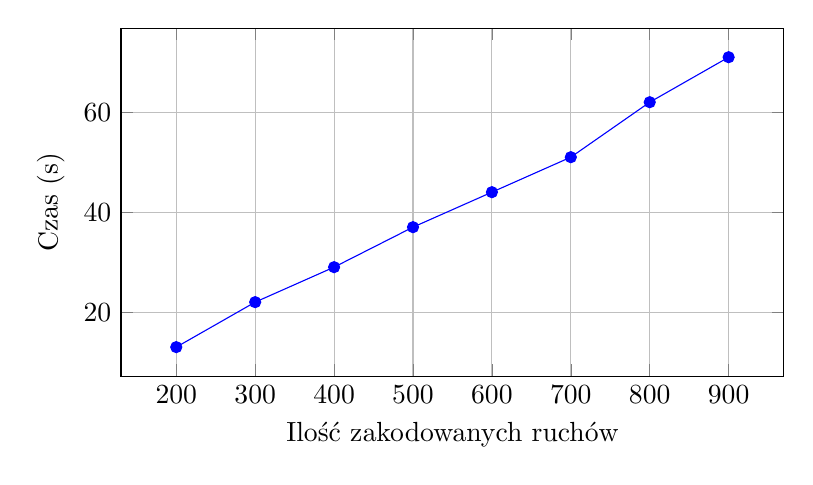
\begin{tikzpicture}
    \begin{axis}[
        xlabel={Ilość zakodowanych ruchów},
        ylabel={Czas (s)},
        grid=major,
        legend pos=north east,
        width=10cm,
        height=6cm
    ]
    \addplot[blue, mark=*] coordinates {
        (200, 13)
        (300, 22)
        (400, 29)
        (500, 37)
        (600, 44)
        (700, 51)
        (800, 62)
        (900, 71)
    };
    \end{axis}
    \end{tikzpicture}
    \caption{Czas wykonania metod concatenate po każdym zakodowaniu gry}
    \label{fig:concatenate_time}
\end{figure}